\documentclass[border=10pt]{standalone}
\usepackage{tkz-graph}
\GraphInit[vstyle = Classic]
\tikzset{
  LabelStyle/.style = { rectangle, rounded corners, 
                        fill = white!50,
                        text = black, font = \small\bfseries },
  VertexStyle/.append style = { inner sep=5pt, fill=white,thick,
                                font = \Large\bfseries, thick},
  EdgeStyle/.append style = {-> , font=\bfseries} }
\thispagestyle{empty}
\begin{document}
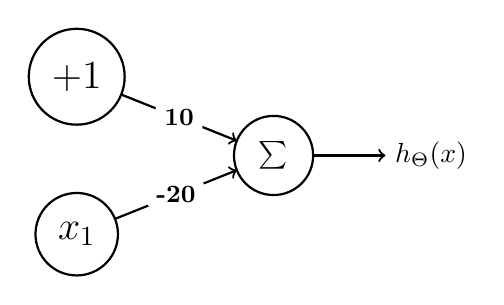
\begin{tikzpicture}
  \SetGraphUnit{45pt}
  \node[VertexStyle](C) at (0,0) {$\sum$}; 
  \node[VertexStyle](A) at (-2.5,1) {$+1$}; 
  \node[VertexStyle](B) at (-2.5,-1){$x_1$};
  \node[draw=none](D) at (2,0){$h_\Theta(x)$};
  %\NOWE(C){A}
  %\WE(C){B}
  \Edge[label = 10](A)(C)
  \Edge[label = -20](B)(C)
  \Edge[](C)(D)
\end{tikzpicture}
\end{document}
